\section{\AP{}Semantic Tree-Width for Simple Queries}
\label{sec:sre}

\todo{small intro}
We devote this section to showing the following result.

% Main theorem : introduced in intro-prelim.tex
\thmSemTwSREpitwo 

% Observe that, for the particular case of an "SRE" $e$, $\+A_e[q,q']$ is also expressible via an "SRE". In fact, "SRE" is "effectively closed under sublanguages". 
Observe that "simple regular expressions" are "closed under sublanguages". Hence, in the light of
\Cref{thm:closure-under-sublanguages}, the "maximal under-approximation" of a {\UCRPQSRE} query by infinitary unions of "CQs" of "tree-width" $k$ is always equivalent to a {\UCRPQSRE} query  of "tree-width" $k$. We will see how the construction of the "maximal under-approximation" of the previous section can be exploited to improve the complexity from "2ExpSpace" down to "PiP2".

\subsection{\AP{}Summary Queries}
We will first show that the "maximal under-approximation" of "tree-width" $k$ of a "UC2RPQ" can be expressed as a union of polynomial sized ``summary'' queries. Each "summary query" represents a union of exponentially-bounded "C2RPQs" sharing some \emph{common structure}. 
"Summary queries" are normal "UC2RPQ" queries extended with some special kind of atoms, called ``"path-$l$ approximations"''. 
Intuitively, they represent a "maximal under-approximation" of "tree-width" $l$ of queries of the form $\bigwedge_i x_i \atom{L_i} y_i$ such that $x_i \neq y_j$ for all $i,j$. 
Path-$l$ approximations may require an exponential size when represented as "UC2RPQs".
%
\AP Formally, a ""path-$l$ approximation"" is a query of the form ``$\intro*\pathl(X, Y, \delta)$''
where: 
\begin{enumerate}
	\item $X$, $Y$, are two disjoint sets of variables of size at most $l$, 
	\item $\delta(\bar z)$ is a conjunction of "atoms" $\bigwedge_{1 \leq i \leq n} A_i$ where $\bar z$ contains all variables of $X \cup Y$,
	\item each $A_i$ is a "C2RPQ" atom of the form $x \atom{L} y$ or $y \atom{L} x$  such that $x \in X$, $y \in Y$, and $L_i$ is a regular language over $\A$.
	%% OLD VERSION:
	% \item $\delta(\bar z)$ is a conjunction of "atoms" $\bigwedge_{1 \leq i \leq n} A_i(x_i,y_i)$ where $\bar z$ contains all variables of $X \cup Y$,
	% \item each $A_i$ is a "C2RPQ" atom of the form $x_i \atom{L} y_i$ or $y_i \atom{L} x_i$  such that $x_i$ is in $X$ and $y_i$ is in $Y$, and $L_i$ is a regular language over $\A$.
\end{enumerate}
We give the semantics of $\pathl(X, Y, \delta)$ in terms of infinitary unions of "C2RPQs".
A query like the one before is defined to be equivalent to the (infinitary) union of all queries $\alpha(\bar z) \in \MUA{\delta}{\Pw[l]}$ such that
\begin{align}
	\text{$\alpha$ has a "path decomposition" of "width" $l$ where $X$ is the root and $Y$ is the leaf,}\AP\label{eq:pathl:rootleafppty}
\end{align}
that is, the root and leaf "bags" contain precisely the vertices of $X$ and $Y$, respectively.
 See \Cref{fig:l-path-example} for an example.
\begin{figure*}
  \centering
  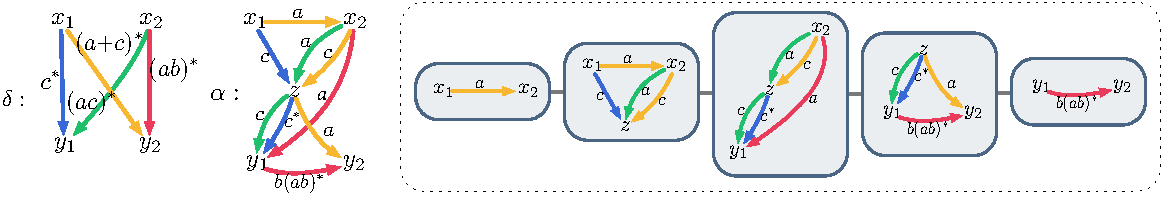
\includegraphics[width = \textwidth]{summary-example.pdf}
  \caption{
	\AP\label{fig:l-path-example}
	Consider the "path-$l$ approximation" $\pathl(\set{x_1,x_2}, \set{y_1,y_2},\delta)$ where $l=2$ and $\delta$ is depicted on the left. Its semantics contains the "approximation" $\alpha(x_1,x_2,y_1,y_2) \in \MUA{\delta}{\Pw[l]}$ depicted in the middle because it has "path decomposition" of "width" $l$ verifying \eqref{eq:pathl:rootleafppty}, as shown on the right.
	}
\end{figure*}

\AP We now simply define a ""$k$-summary query"" as a "C2RPQ" extended with "path-$l$ approximation" atoms for any $l\leq k$, with the expected semantics.
A \AP""refinement@@summary"" of a "$k$-summary query" is any "C2RPQ" obtained by
replacing "atoms" with "atom refinements", and 
each "path-$l$ approximation" $\pathl(X, Y, \delta)$ with any
$\alpha(\bar z) \in \MUA{\delta}{\Pw}$ verifying \eqref{eq:pathl:rootleafppty}. By definition,
a "database@@graph" satisfies a "$k$-summary query" if and only if it
satisfies one of its "refinements@@summary".

A \AP ""tree decomposition@@summary"" of a "$k$-summary query" $\gamma$ consists of
a pair $\tup{\?T, \bagmap}$ with $\bagmap: \vertex{\?T} \to \pset{\vars{\gamma}}$
such that:
\begin{itemize}
	\item for every classical "atom" $x \atom{L} y$ in $\gamma$,
		there is a "bag" $b \in T$ such that $\{x,y\} \subseteq \bagmap(b)$;
	\item for every "path-$l$ approximation" $\pathl(X, Y, \delta)$ in $\gamma$,
		there are two adjacent "bags" $b, b' \in T$ such that $X \subseteq \bagmap(b)$
		and $Y \subseteq \bagmap(b')$.
\end{itemize}
The "width" is defined as usual. Then, by
\Cref{fact:refinement-tw}, we obtain the following upper bound.

\begin{fact}
	\AP\label{fact:tree-width-summary}
	For any $k\geq 2$, any "refinement@@summary" of a "$k$-summary query" with
	a "tree decomposition@@summary" of "width" at most $k$ is a "C2RPQ" of "tree-width" at most $k$.
\end{fact}

Lastly, a \AP""homomorphism@@summary"" from a "C2RPQ"
$\gamma(\bar z) = \bigwedge_{i} x_i \atom{L_i} y_i$
to a "summary query" $\delta(\bar z') =
\bigl( \bigwedge_{j} x'_j \atom{L'_j} y'_j \bigr)
\wedge \bigl( \bigwedge_{j'} \pathl(X_{j'}, Y_{j'}, \delta_{j'}) \bigr)$
consists of a mapping $\fun$ from variables of $\gamma$ to variables of $\delta$
such that $f(\bar z) = \bar z'$, and for each $i$,
there is an atom $f(x_i) \atom{L_i} f(y_i)$ in $\delta$.
Note that if there is a homomorphism from $\gamma(\bar z)$ to $\delta(\bar z')$,
then $\delta(\bar z') \contained \gamma(\bar z)$.

Let us fix $\+L$ to be any class  "closed under sublanguages". For every $\gamma \in \CtwoRPQ(\+L)$, we define \AP $\intro*\Qapp$ as the set of all "$k$-summary queries" $\alpha$ such that:
\begin{enumerate}[label=\roman*.]
	\item $\alpha$ has a "fine tagged tree decomposition" $\tup{\?T, \bagmap}$ of "width" at most $k$,
	\item there exists a "strong onto" "homomorphism@@summary" from a "refinement" $\rho$ of $\gamma$ to $\alpha$, 
	\item $T$ has at most $2\nbatoms{\gamma}$ leaves, and every
		"non-branching path" of $T$ consisting only of "non-atomic" "bags" must contain at most two "non-full bags".
\end{enumerate}
Note that since $\alpha$ is a homomorphic image a "refinement" of $\gamma$,
and since $\+L$ is "closed under sublanguages", then $\alpha$ has only $\+L$-labelled "atoms".

\begin{lemma}\AP\label{lemma:MUAk-union-of-polysized-summary-test-np}
    \AP Let $k \geq 2$. For every \textbf{finite} class $\+L$ "closed under sublanguages",
	and for every $\gamma \in \CtwoRPQ(\+L)$, 
	% define \AP $\intro*\Qapp$ as the set of all
	% "$k$-summary queries" $\alpha$ such that:
	% \begin{enumerate}[label=(\roman*)]
	% 	\item $\alpha$ has a "fine tagged tree decomposition" $\tup{\?T, \bagmap}$ of "width" at most $k$,
	% 	\item there exists a "homomorphism@@summary" from a "refinement" $\rho$ of $\gamma$
	% 		to $\alpha$, and
	% 	\item $T$ has at most $2\nbatoms{\gamma}$ leaves, and every
	% 		"non-branching path"
	% 		of $T$ consisting only of "non-atomic" "bags" must contain at most two "non-full bags".
	% \end{enumerate}
	% Then, 
	we have:
	\begin{enumerate}
		\itemAP \label{lemma:MUAk-union-of-polysized-summary-test-np:1} $\Qapp \semequiv \MUA{\gamma}{\Tw}$,
		\itemAP \label{lemma:MUAk-union-of-polysized-summary-test-np:2} $\Qapp$ is a union of polynomial-sized "$k$-summary queries" having only
			$\+L$-labelled "atoms", and
		\itemAP \label{lemma:MUAk-union-of-polysized-summary-test-np:3} one can test in "NP" if a "summary query" is part of this union.
	\end{enumerate}
\end{lemma}
% \begin{proof}[Informal proof]
%   As corollary of the proof of \Cref{lemma:bound_size_refinements}, we can assume to have 
%   $\MUA{\gamma}{\Tw}$ expressed as a union of $\CtwoRPQ(\+L)$ with a "nice tree decomposition" of "width" $k$ with a linear number of leaves, and hence it suffices to replace "non-branching paths" with "path-$l$ approximations".
%   Concretely, for any such "C2RPQ" $\alpha$ having a witnessing "tree decomposition" with a long "non-branching path", the tree must contain a sub-path whose every bag is "non-atomic", and such that it starts and ends in "bags" of size at most $k$ (by the "niceness" property).
%   Such a "non-atomic" "non-branching path" can be ``compressed'' by replacing the subquery corresponding to the path with a corresponding "path-$l$ approximation" query. The resulting summary query will "contain" $\alpha$ and in turn be "contained" in $\gamma$. Simultaneously applying such replacement to all "non-atomic" "non-branching paths" of maximal length then yields a polynomial sized "summary query".
  
%   Further, given a "$k$-summary query" $\sigma$, one can test in "NP" whether there exists an element of $\MUAHom{\gamma}{\Tw}$ that leads to such "summary query" by the process just mentioned. This is done by first checking that $\sigma$ is of the ``right shape'' (essentially a query of tree-width $k$ when disregarding the "path-$l$ approximation" atoms), and that it is "contained" in $\gamma$ via a polynomial "refinement" $\rho \in \Refin(\gamma)$ and a "strong onto homomorphism" to the query resulting from replacing $\pathl(X,Y,\delta)$ atoms with $\delta$ in $\sigma$.
%   % \ifspaceallows{\newline\indent Further, given a "$k$-summary query" $\sigma$, one can test in "NP" whether there exists an element of $\MUAHom{\gamma}{\Tw}$ that leads to such "summary query" by the process just mentioned. This is done by first checking that $\sigma$ is of the ``right shape'' (essentially a query of tree-width $k$ when disregarding the "path-$l$ approximation" atoms), and that it is "contained" in $\gamma$ via a polynomial "refinement" $\rho \in \Refin(\gamma)$ and a "strong onto homomorphism" to the query resulting from replacing $\pathl(X,Y,\delta)$ atoms with $\delta$ in $\sigma$.}{The test for "NP" can be found in the Appendix.}
% \end{proof}
\begin{proof}
	Point \eqref{lemma:MUAk-union-of-polysized-summary-test-np:2} follows directly from the definition: there are few branches in the decomposition, branches are short, and each "bag" cannot contain more than $(k+1)^2 \cdot |\+L|$ "atoms" labelled with $\+L$-languages.

	For point \eqref{lemma:MUAk-union-of-polysized-summary-test-np:3}, recall that one can check if a query has "tree-width" at most $k$ in linear time, "eg" using Bodlaender's algorithm (\Cref{prop:bodlaender}).

	% Points \eqref{lemma:MUAk-union-of-polysized-summary-test-np:2} and \eqref{lemma:MUAk-union-of-polysized-summary-test-np:3} follow directly from the definition---recall
	% that one can check if a query has "tree-width" at most $k$ in linear time
	% with Bodlaender's algorithm (\Cref{prop:bodlaender}).

	To prove \eqref{lemma:MUAk-union-of-polysized-summary-test-np:1}, notice first that 
	$\Qapp \contained \MUA{\gamma}{\Tw}$ as a consequence
	of \Cref{fact:tree-width-summary}.

	For the converse "containment", we use \Cref{coro:equivalence_under_approx_homomorphism_twk}
	and prove instead $\MUAHom{\gamma}{\Tw} \contained \Qapp$.
	Observe that, as corollary of the proof of \Cref{lemma:bound_size_refinements}, we can assume to have 
	$\MUAHom{\gamma}{\Tw}$ expressed as a union of $\CtwoRPQ(\+L)$ with a "fine tagged tree decomposition" of "width" $k$ with at most $2\nbatoms{\gamma}$ leaves, and hence it suffices to replace each "non-branching paths" having "non-atomic" bags with "path-$l$ approximations".

	Indeed, fix a "fine tagged tree decomposition" and a "trio"
	$\fun\colon \rho \surj \alpha$. Given a long "non-branching path" from "bag" $b_X$ with
	variables $X$ to a "bag" $b_Y$ with variables $Y$,
	such that $b_X$ and $b_Y$ are "non-full", and no "bag" in between is "atomic",
	define $X' \defeq X \setminus Y$ and $Y' \defeq Y \setminus X$.
	Consider the set $\+S$ of "atoms" $u \atom{L} v$ of $\gamma$, such that the "path induced"
	$\bigl( {b_i \choose z_i} \bigr)_i$ by the "refinement", say
	\[
		u = w_0 \atom{L_0} w_1 \atom{L_1} \cdots \atom{L_n} w_n	= v
	\]
	of $u \atom{L} v$ in $\rho$ 
	goes through $b_X$ at some variable of $X'$ and through $b_Y$ at some variable
	of $Y'$, in the sense that $b_i = b_X$ and $z_i \in X'$ for some $i$,
	and $b_j = b_Y$ and $z_j \in Y'$ for some $j$.
	There exist $i', j'$ such that $f(w_{i'}) = z_i$ and $f(w_{j'}) = z_j$,
	and "wlog" $i' < j'$.
	Now let $\alpha'$ be the query obtained from $\alpha$ by removing all "atoms" tagged in a bag between $b_X$ and $b_Y$, and add a "path-$l$ approximation" query
	\[
		\pathl(X', Y', \delta)
	\]
	where $\delta$ is the conjunction over $u \atom{L} v \in \+S$ of
	$w_{i'} \atom{\contract{L_{i'}\cdots L_{j'}}} w_{j'}$.
	Repeat this operation for every non-trivial "non-branching path" with
	"non-atomic" "bags". We obtain $\alpha'' \in \Qapp$ "st"
	$\alpha \contained \alpha''$, which concludes the proof
	that $\MUAHom{\gamma}{\Tw} \contained \Qapp$.
\end{proof}


\subsection{\AP{}Semantic Tree-Width Problem}
With the previous results in place, we now show that the semantic tree-width $k$ problem is in {"PiP2"} for \UCRPQSRE, for every $k>1$.

\thmSemTwSREpitwo*
%Theorem: For every $k>1$, the "semantic tree-width $k$ problem" for {\UCRPQSRE} is in "PiP2".
\begin{proof}
  It suffices to show the statement for any $\CRPQSRE~\gamma$. Remember that $\gamma$ is of "semantic tree-width" $k$ if, and only if, $\gamma \contained \Qapp$. The first ingredient to this proof is the fact that this "containment" has a polynomial counterexample property.
%   \begin{restatable}{clm}{claimpolysizedcounterexamplesre}
%     \AP\labelwithproof{claim:poly-sized-counterexample-sre}
%     If $\gamma \notcontained \Qapp$ then there is a polynomial-sized "expansion" $\anexpansion$ of $\gamma$ such that $\anexpansion \notcontained \Qapp$.
%   \end{restatable}
  
  \begin{claim}\AP\label{claim:poly-sized-counterexample-sre}
    If $\gamma \notcontained \MUAHom{\gamma}{\Tw} $ then there is a polynomial-sized "expansion" $\anexpansion$ of $\gamma$ such that $\anexpansion \notcontained \MUAHom{\gamma}{\Tw} $.
  \end{claim}
  \begin{proof}
    \newcommand{\Qalt}{\+U}
    \AP
    Let us call any atom with a language of the form $a^*$ a ""recursive atom"", and any other atom a ""non-recursive atom"".
    Let $n$ be the number of "non-recursive atoms" of $\gamma$. Hence, any refinement $\rho \in \Refin(\gamma)$ has $n$ atoms deriving from "non-recursive@@nrat" "atom refinements", all the remaining ones derive from "recursive@@rat" "atom refinements".

    We will work with the infinitary union of "conjunctive queries"
	\[\Qalt\defeq\MUAHom{\gamma}{\Tw} \cap \textnormal{"CQ"}.\]
	Note that $\Qalt=\set{ \alpha \in \textnormal{"CQ"} \mid \alpha \in \Tw \text{ and there is } \anexpansion \in \Exp(\gamma) \text{ "st" } \anexpansion \surj \alpha }$.
    It is easy to see that $\Qalt \semequiv \MUAHom{\gamma}{\Tw}$ as a consequence of \Cref{fact:refinement-tw}.
	% (and thus $\Qalt \semequiv \Qapp$).
    By \Cref{prop:cont-char-exp-st}, we have $\gamma \notcontained \Qalt$ if, and only if, there is some "expansion" $\anexpansion$ of $\gamma$ such that $\anexpansion \notcontained \Qalt$. In turn, this happens if, and only if, there is no $\delta \in \Qalt$ such that $\delta \homto \anexpansion$.
    
    Take any such counterexample $\anexpansion$ of minimal size (in number of atoms). We show that for any "internal path" of $\anexpansion$ of the shape
    \[\pi = x_0 \atom{a} x_1 \atom{a} x_1 \dotsb x_{m-1}\atom{a} x_m,\]
    we have $m \leq n+1$. Hence, since $\anexpansion$ is an "expansion" of a {\CRPQSRE}, this means that the size of each \AP""atom expansion""---namely an "expansion" obtained from a query by only expanding one "atom"---of $\anexpansion$ is linearly bounded in the size of $\gamma$, and thus that $\anexpansion$ is quadratically bounded.

    By means of contradiction, if $m > n+1$ consider the "expansion" $\anexpansion'$ resulting from ``shrinking'' the path $\pi$ to a path $\pi'$ of length $n+1$. Hence, $\anexpansion'$ is smaller than $\anexpansion$, and since $\anexpansion$ was assumed to be minimal, $\anexpansion'$ cannot be a counterexample. Thus, there is some $\delta \in \Qalt$ such that $\fun_1:\delta \homto \anexpansion'$ for some "homomorphism" $\fun_1$. Further, by definition of $\Qalt$, we have $\fun_2 : \anexpansion'' \surj \delta$ for some $\anexpansion'' \in \Exp(\gamma)$. Consider then the composition $\anexpansion'' \surj \delta \homto \anexpansion'$ of $\fun_2$ with $\fun_1$ and let us call it $g: \anexpansion'' \homto \anexpansion'$. By definition of $n$ there must be at least one atom $x_i \atom{a} x_{i+1}$ of the shrunken path $\pi'$ of $\anexpansion'$ which either 
		(i) is not in the image of $\fun_1$, or 
		(ii) all its $g$-preimages proceed from "atoms" $z \atom{a} z'$ of $\anexpansion''$ which are in the "expansions" of "recursive atoms" of $\gamma$. 
	We show that, in both cases, we can replace $x_i \atom{a} x_{i+1}$ with a path of $a$'s of any arbitrary length $l>0$, obtaining a "conjunctive query" $\anexpansion'_{+l}$  which
	is---still---not a counterexample.  In the first case (i), we actually obtain that $\delta \homto \anexpansion'_{+l}$. In the second case (ii), we have to replace each atom $z \atom{a} z'$ in the $g$-preimage of $x_i \atom{a} x_{i+1}$ in $\anexpansion''$ by an $a$-path of length $l$, obtaining some "expansion" $\anexpansion''_{+l}$ of $\gamma$. We also replace each atom in the $\fun_1$-preimage of $x_i \atom{a} x_{i+1}$ by an $a$-path of length $l$ obtaining some $\delta_{+l}$ such that $\anexpansion''_{+l} \surj \delta_{+l} \homto \anexpansion'_{+l}$. Further, $\delta_{+l} \in \Tw$ since $\Tw$ is closed under "refinements" by \Cref{fact:refinement-tw}.
    In both cases this shows that $\anexpansion'_{+l}$ is \emph{not} a counterexample. 
	In particular, for $l=m-n-1$, we have $\anexpansion'_{+l}=\anexpansion$, and this would contradict the fact that $\anexpansion$ is a counterexample.
	Therefore, there exists a counterexample of polynomial (quadratic) size whenever $\gamma \notcontained \MUAHom{\gamma}{\Tw}$.
  \end{proof}
%   This is because any path $x_0 \atom{a}  \dotsb \atom{a} x_m$ in an expansion $\anexpansion$ of $\gamma$ such that $m > \nbatoms{\gamma}$ and $\anexpansion \contained \Qapp$ can be `pumped' to an even longer path of any length greater than $m$ obtaining another expansion $\anexpansion'$ such that $\anexpansion' \contained \Qapp$. This implies that a minimal counterexample must be of polynomial size. \ifspaceallows{The proof uses rather standard techniques and can be found in \Cref{appendix:sre}.}{}
  The second ingredient is that testing whether a "CQ" is a counterexample is in "coNP".

  \begin{claim}\AP\label{claim:cq-in-Qapp-np}
    The problem of testing, given a "C2RPQ" $\gamma$ and a "CQ" $\xi$, whether $\xi \contained \Qapp$, is in "NP".
  \end{claim}
  % \begin{proof}[Informal proof]
  %   We first guess a polynomial-sized "$k$-summary query" $\delta_{\textup{zip}}$ and test in "NP" that it is part of $\Qapp$ by \Cref{lemma:MUAk-union-of-polysized-summary-test-np}. 
  %   We now guess a valuation $\mu :  \vars{\delta_{\textup{zip}}} \to \vars{\gamma}$ and test that it is a "homomorphism" $\anexpansion \homto \gamma$, where $\anexpansion$ is an expansion of the "CRPQ" resulting from discarding the "path-$l$ approximation" atoms of $\delta_{\textup{zip}}$, which can be done in \nl. It remains to check that each atom $\pathl(X,Y,\hat \delta)$ of $\delta$ has an "expansion" $\hat\anexpansion$ such that $h : \hat\anexpansion \homto \gamma$ for a "homomorphism" such that $h(x)=\mu(x)$ for all $x \in X \cup Y$. This can be done via an \nl algorithm using $l+1$ pointers to traverse the "width"-$l$ "fine" "path decomposition" of $\hat\anexpansion$, simultaneously guessing $\hat\anexpansion$, the "expansion" of $\gamma$ which homomorphically maps to $\hat\anexpansion$, and the valuation of $h$.
  % \end{proof}
  \begin{proof}
        We first guess a polynomial-sized "$k$-summary query" $\delta_{\textup{zip}}$ and test in "NP" that it is part of $\Qapp$ by \Cref{lemma:MUAk-union-of-polysized-summary-test-np}. 
        Let us call $\Delta$ be the equivalent {\UCRPQSRE} query, given by \Cref{lemma:MUAk-union-of-polysized-summary-test-np} \textit{cum} \Cref{lemma:bound_size_refinements}.
        We have to check that there is some "expansion" $\delta$ of $\Delta$ such that there is a "homomorphism" $\delta \homto \xi$. 
        We first guess a valuation $\mu :  \vars{\delta_{\textup{zip}}} \to \vars{\xi}$.
        Now it remains to check that:
        \begin{enumerate}
          \item For every "CRPQ" atom $x \atom{a^*} y$ of $\delta_{\textup{zip}}$ there is an $a$-path in $\xi$ from $\mu(x)$ to $\mu(y)$.
          \item Every "path-$l$ approximation" $\pathl(X, Y, \bigwedge_{1 \leq i \leq n} A_i(x_i,y_i))$ of $\delta_{\textup{zip}}$ contains a "CQ" $\delta_{\textup{path}}$  admitting a "path decomposition" of "width" $l$ which starts with the bag $X$ and ends with $Y$. And further, there is a homomorphism $h: \delta_{\textup{path}}  \homto \xi$ which coincides with $\mu$ on variables $X \cup Y$.
        \end{enumerate}
        Observe that  these two properties hold true if, and only if, there is some "expansion" $\delta$ of $\Delta$ such that $\delta \homto \gamma$.
        It is clear the first point can be achieved in polynomial time (actually, in "NL") since it is a simple reachability query. 
        The second point can also be achieved in polynomial time (or in "NL"), since the "fine" "path decomposition" of "width" $l$ can be guessed on-the-fly using $l+1$ pointers to the variables of $\gamma$ ("cf" \Cref{lemma:evaluation-bounded-pathwidth}). An "NL" algorithm can advance down the "path decomposition" while simultaneously
        \begin{enumerate}
          \item guessing the "conjunctive query" $\delta_{\textup{path}}$ via its "fine" "path decomposition" of "width" $k$,
          \item checking that there is a partial "homomorphism" to $\gamma$ ("ie", a "homomorphism" from the subquery of $\gamma$ restricted to current "bag"'s variables to $\gamma$),
          \item ensuring that the "CQ" $\delta_{\textup{path}}$ being built is an element of
		  \[\pathl(X, Y, \bigwedge_{1 \leq i \leq n} A_i(x_i,y_i)),\] which requires to also guess a homomorphism $\rho \homto \delta_{\textup{path}}$ from a refinement $\rho$ of $\bigwedge_{1 \leq i \leq n} A_i(x_i,y_i)$.
        \end{enumerate}
        Further, a simple test can ensure that the first and last bags of the decomposition  coincide with the guessed assignment $\mu$.
        Since the number of pointers (bounded by $k+1$) is fixed, this subroutine is in "NL", and hence in polynomial time. This yields an "NP" algorithm for testing $\xi \contained \Qapp$.
  \end{proof}


  As a consequence of the two claims, we obtain a "SigmaP2"~algorithm for non-containment of $\gamma \contained \Qapp$: We first guess an "expansion" $\anexpansion$ of $\gamma$ of polynomial size, and we then test $\anexpansion \notcontained \Qapp$ in "coNP". This gives a {"PiP2"} algorithm for the "semantic tree-width $k$ problem", which is correct by
  \Cref{lemma:MUAk-union-of-polysized-summary-test-np,claim:poly-sized-counterexample-sre}.
\end{proof}